\documentclass[sigconf]{acmart}

\usepackage{tikz}
\usetikzlibrary{calc,shapes.multipart,chains,arrows,arrows.meta}
\usepackage{minted}

\newcommand{\green}[1]{\color{green}\color{.!80!black}{#1}}
\newcommand{\red}[1]{\color{red}{#1}}
\newcommand{\hsinl}[1]{\mintinline[breaklines]{haskell}{#1}}
\newcommand{\code}[1]{\texttt{#1}}
\newcommand{\ThunkLang}{\code{ThunkLang}}
\newcommand{\EnvLang}{\code{EnvLang}}
\newcommand{\StateLang}{\code{StateLang}}
\newcommand{\FlatLang}{\code{FlatLang}}
\newcommand{\ClosLang}{\code{ClosLang}}

\begin{document}

\title{Verified Compilation of Thunks in PureCake}

\author{Nikolaos Alexandris}
\orcid{0009-0002-2856-146X}
\affiliation{%
  \institution{National and Kapodistrian University of Athens}
  \department{Department of Informatics and Telecommunications}
  \city{Athens}
  \country{Greece}}
\email{nalex@di.uoa.gr}

\author{Magnus O. Myreen}
\affiliation{%
  \institution{Chalmers University of Technology}
  \city{Gothenburg}
  \country{Sweden}}
\email{myreen@chalmers.se}

\begin{abstract}
  Programming languages that are lazy by default, such as Haskell, need their
  compilers to handle thunks as efficiently as possible to minimise the lazy
  behaviour's impact on the runtime. This is achieved both during compile time
  by avoiding the generation of unnecessary thunks, and during the runtime by
  replacing evaluated thunks with their values during garbage collection. In
  this work, we refine the representation of thunks in the PureCake verified
  compiler for pure lazy languages, we introduce thunks as first-class values in
  PureCake's compilation target CakeML, and we adapt CakeML's garbage collector
  to optimise their runtime handling.
\end{abstract}

\keywords{Compiler Verification, Lazy Functional Programming, Theorem Proving,
          Haskell, HOL4, PureCake, CakeML}

\begin{teaserfigure}
  \centering
  \begin{tikzpicture}
    \node (fig1) {
        \begin{tikzpicture}[
    list/.style={
      rectangle split, rectangle split parts=2, draw,
      rectangle split horizontal},
    cell/.style={
      rectangle split, rectangle split parts=2, draw,
      rectangle split horizontal,fill=cyan,fill opacity=0.5, text opacity=1,
      draw opacity=1},
    box/.style={rectangle, draw, minimum width=0.5cm, minimum height=0.5cm},
    arr/.style = {draw=#1, thick,
                 {Circle[length=6pt,sep=-3pt]}-{Stealth[width=6pt]}},
    >=stealth, node distance=2.5cm]
  \node[rectangle,draw] (XSP) {};
  \node[rectangle] (XS)[left of=XSP,xshift=2cm] {\texttt{xs}};
  \node[list] (E1)[above of=XSP,xshift=0.5cm,yshift=-1.5cm] {
    \green{\texttt{E}}};
  \node[list] (E2)[right of=E1,xshift=-1cm] {
    \green{\texttt{E}}};
  \node[list] (E3)[right of=E2,xshift=-1cm] {
    \green{\texttt{E}}};
  \node[list] (E4)[right of=E3,xshift=-1cm]
    {\green{\texttt{E}} \nodepart{second} \texttt{[]}};
  \node[cell] (C1)[above of=E1,xshift=0.7cm,yshift=-1.5cm] {};
  \node[cell] (C2)[right of=C1,xshift=-1cm] {};
  \node[cell] (C3)[right of=C2,xshift=-1cm] {};
  \node[list] (NE2)[above of=C2,yshift=-1.5cm]
    {\green{\texttt{E}} \nodepart{second} 2};
  \node[list] (NE1)[above of=C1,yshift=-1.5cm]
    {\green{\texttt{E}} \nodepart{second} 1};
  \node[list] (NE3)[above of=C3,yshift=-1.5cm]
    {\green{\texttt{E}} \nodepart{second} 3};
  \path[arr] (XSP.center) -- (E1);
  \path[arr] (E1.two north |- E1.two east) -- (C1);
  \path[arr] (E2.two north |- E2.two east) -- (C2);
  \path[arr] (E3.two north |- E3.two east) -- (C3);
  \path[arr] (C1.two north |- C1.two east) -- (E2);
  \path[arr] (C2.two north |- C2.two east) -- (E3);
  \path[arr] (C3.two north |- C3.two east) -- (E4);
  \path[arr] (C1.one north |- C1.one east) -- (NE1);
  \path[arr] (C2.one north |- C2.one east) -- (NE2);
  \path[arr] (C3.one north |- C3.one east) -- (NE3);
\end{tikzpicture}

    };

    \node (fig2) [right=3cm of fig1] {
        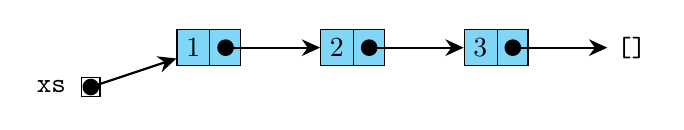
\begin{tikzpicture}[
    list/.style={
      rectangle split, rectangle split parts=2, draw,
      rectangle split horizontal},
    cell/.style={
      rectangle split, rectangle split parts=2, draw,
      rectangle split horizontal,fill=cyan,fill opacity=0.5, text opacity=1,
      draw opacity=1},
    box/.style={rectangle,draw},
    boxinv/.style={rectangle},
    arr/.style = {draw=#1, thick,
                 {Circle[length=6pt,sep=-3pt]}-{Stealth[width=6pt]}},
    >=stealth, start chain]
  \node[cell,on chain] (B) {$1$};
  \node[cell, on chain] (C) {$2$};
  \node[cell, on chain] (D) {$3$};
  \node[on chain] (E) {\texttt{[]}};
  \node[box] (XSP)[left of=B,xshift=-0.5cm,yshift=-0.5cm] {};
  \node[boxinv] (XS)[left of=XSP,xshift=0.5cm] {\texttt{xs}};
  \path[arr=black] (XSP.center) -- (B);
  \path[arr=black] (B.two north |- B.two east) -- (C);
  \path[arr=black] (C.two north |- C.two east) -- (D);
  \path[arr=black] (D.two north |- D.two east) -- (E);
\end{tikzpicture}

    };

    \coordinate (arrow-start) at ([xshift=0.8cm]fig1.east);
    \coordinate (arrow-end)   at ([xshift=-0.3cm]fig2.west);

    \draw[->, thick] (arrow-start) -- (arrow-end);
\end{tikzpicture}

  \caption{GC inlining of a list of evaluated thunks.}
  \Description{GC inlining of a list of evaluated thunks.}
  \label{fig:teaser}
\end{teaserfigure}

\maketitle

\section{Introduction}

PureCake is an end-to-end formally verified compiler for PureLang, a
Haskell-inspired lazy purely functional programming language with monadic
effects. The compiler's frontend implements a Haskell-like indentation sensitive
syntax, a type checker, and demand analysis. Its backend consists of three
intermediate languages that it uses to gradually transform a syntax tree of its
source language to CakeML's source language.

CakeML is a functional programming language based on a substantial subset of
Standard ML and an ecosystem of proofs and tools built around the language. The
ecosystem includes a verified compiler from its source language to assembly.
PureCake uses this compiler to create the end-to-end verified compilation from
PureLang to assembly. This process is similar to writing a Haskell compiler by
transforming the Haskell source code to Standard ML source code, and then
calling the Standard ML compiler to lower the generated syntax tree to machine
code.
\begin{figure}[h]
  \centering
  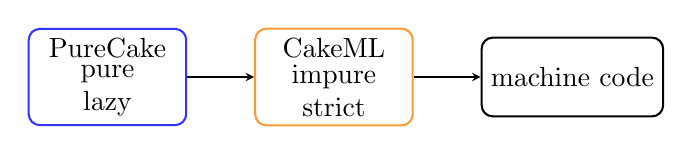
\begin{tikzpicture}
  \tikzstyle{box} = [
    rectangle, rounded corners, minimum width=2cm, minimum height=1cm,
    text centered, draw=black, line width=0.75pt
  ]
  \node (box1) [box, draw=blue!80] {
    \shortstack{PureCake \\ pure \\ lazy}
  };
  \node (box2) [box, right=0.85cm of box1, draw=orange!80] {
    \shortstack{CakeML \\ impure \\ strict}
  };

  \node (box3) [box, right=0.85 of box2] {
    machine code
  };

  \draw[-stealth] (box1.east) -- (box2.west) node[]{};
  \draw[-stealth] (box2.east) -- (box3.west) node[]{};
\end{tikzpicture}

  \caption{Overview of end-to-end compilation process.}
  \Description{Overview of end-to-end compilation process.}
  \label{fig:comp-process}
\end{figure}

PureLang and CakeML's source languages differ in semantics in two major ways:
purity and evaluation strategy. In order for the PureCake compiler to transform
a PureLang program to a CakeML one, it needs to convert the lazy (call-by-name)
evaluation to strict (call-by-value) evaluation. This is traditionally achieved
in lazy language compilers by introducing thunks. Consider the simple PureLang
function definition \hsinl{suc n = n + 1}. Semantically, when a call like
\hsinl{suc (f x)} happens, the \code{f x} call is only performed when the
\code{+} operator demands its value in the body of \hsinl{suc}. In order to
transform the program's evaluation strategy, the compiler extends the language
with two special expressions: \code{delay} and \code{force}. Here, \code{delay}
wraps an expression in a thunk, and \code{force} queries a thunk for its value.
Therefore, the \hsinl{suc (f x)} lazy call could be simulated in a strict
language by transforming the call to \hsinl{(force suc) (delay ((force f) (delay
x)))} and the function to \hsinl{suc n = (force n) + 1}.

PureCake achieves the evaluation strategy transformation by passing the source
program through a series of intermediate languages, at each step changing the
semantics of the language to bridge the gap between PureCake and CakeML's
semantics. The three intermediate languages are \ThunkLang{}, \EnvLang{}, and
\texttt{State\allowbreak Lang}.
\begin{figure}[h]
  \centering
  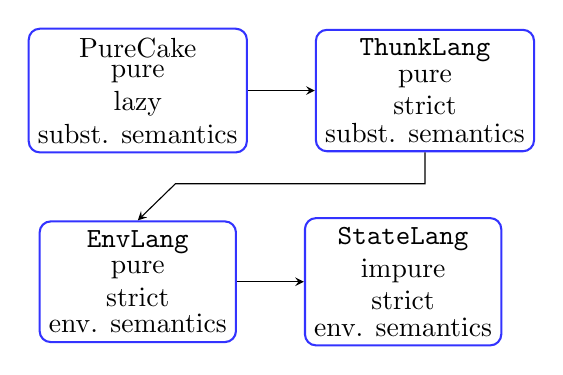
\begin{tikzpicture}
  \tikzstyle{box} = [
    rectangle, rounded corners, minimum width=2cm, minimum height=1cm,
    text centered, draw=blue!80, line width=0.75pt
  ]
  \node (box1) [box] {
    \shortstack{PureCake \\ pure \\ lazy \\ subst. semantics}
  };
  \node (box2) [box, right=0.85cm of box1] {
    \shortstack {
      \texttt{ThunkLang} \\ pure \\ strict \\ subst. semantics
    }
  };
  \node (box3) [box, below=0.85cm of box1] {
    \shortstack{\texttt{EnvLang} \\ pure \\ strict \\ env. semantics}
  };
  \node (box4) [box, right=0.85cm of box3] {
    \shortstack {
      \texttt{StateLang} \\ impure \\ strict \\ env. semantics
    }
  };
  \draw[-stealth] (box1.east) -- (box2.west) node[]{};
  \draw[-stealth] (box2.south) -- ++(0,-0.4cm) -- ++(-3.17cm,0) -- (box3.north) node[]{};
  \draw[-stealth] (box3.east) -- (box4.west) node[]{};
\end{tikzpicture}

  \caption{Overview of PureCake's compilation process.}
  \Description{Overview of PureCake's compilation process.}
  \label{fig:comp-process-pure}
\end{figure}

In \ThunkLang{}, the \code{delay} and \code{force} operators are introduced and
placed around the appropriate expressions as described above, and the evaluation
strategy is converted to call-by-value. While this is semantically enough, it
would be inefficient in practice. In \ThunkLang{}, when a thunk is forced
multiple times, its contained expression will be evaluated for each \code{force}
separately. Since PureCake is a pure language, we know that the value of the
thunk will always be the same regardless of when we evaluate it. So, ideally, we
should only compute it once and then memoise its value for the rest of the
\code{force}s.

This problem is solved in \StateLang{}. \StateLang{}'s semantics employ a
mutable memory called a store. Each time a \code{delay} is executed, a thunk is
produced and appended to the store along with a flag stating that the thunk has
not yet been evaluated. Then, the first \code{force} demanding the thunk's value
will get a reference to the thunk in the store and evaluate its expression. It
will then set the flag to state that the thunk has been evaluated, and overwrite
the unevaluated expression with the result it computed. Any subsequent
\code{force} will then directly use the value instead of re-computing the
expression.

Thunks are the core of lazy behaviour in programming languages like PureCake and
Haskell, and thus their semantics should be as well defined as possible, and
their runtime behaviour optimised. In this work we focus on three things to
achieve these goals in PureCake:
\begin{itemize}
\item Strengthening the semantics of thunks in PureCake;
\item Adding thunks as first-class constructs to CakeML;
\item Optimising the runtime handling of thunks.
\end{itemize}

\section{Template Overview}
\label{sec:purecake}
As noted in the introduction, the ``\verb|acmart|'' document class can
be used to prepare many different kinds of documentation --- a
double-anonymous initial submission of a full-length technical paper, a
two-page SIGGRAPH Emerging Technologies abstract, a ``camera-ready''
journal article, a SIGCHI Extended Abstract, and more --- all by
selecting the appropriate {\itshape template style} and {\itshape
  template parameters}.

This document will explain the major features of the document
class. For further information, the {\itshape \LaTeX\ User's Guide} is
available from
\url{https://www.acm.org/publications/proceedings-template}.

\subsection{Template Styles}

The primary parameter given to the ``\verb|acmart|'' document class is
the {\itshape template style} which corresponds to the kind of publication
or SIG publishing the work. This parameter is enclosed in square
brackets and is a part of the {\verb|documentclass|} command:
\begin{verbatim}
  \documentclass[STYLE]{acmart}
\end{verbatim}

Journals use one of three template styles. All but three ACM journals
use the {\verb|acmsmall|} template style:
\begin{itemize}
\item {\texttt{acmsmall}}: The default journal template style.
\item {\texttt{acmlarge}}: Used by JOCCH and TAP.
\item {\texttt{acmtog}}: Used by TOG.
\end{itemize}

The majority of conference proceedings documentation will use the {\verb|acmconf|} template style.
\begin{itemize}
\item {\texttt{sigconf}}: The default proceedings template style.
\item{\texttt{sigchi}}: Used for SIGCHI conference articles.
\item{\texttt{sigplan}}: Used for SIGPLAN conference articles.
\end{itemize}

\subsection{Template Parameters}

In addition to specifying the {\itshape template style} to be used in
formatting your work, there are a number of {\itshape template parameters}
which modify some part of the applied template style. A complete list
of these parameters can be found in the {\itshape \LaTeX\ User's Guide.}

Frequently-used parameters, or combinations of parameters, include:
\begin{itemize}
\item {\texttt{anonymous,review}}: Suitable for a ``double-anonymous''
  conference submission. Anonymizes the work and includes line
  numbers. Use with the \texttt{\string\acmSubmissionID} command to print the
  submission's unique ID on each page of the work.
\item{\texttt{authorversion}}: Produces a version of the work suitable
  for posting by the author.
\item{\texttt{screen}}: Produces colored hyperlinks.
\end{itemize}

This document uses the following string as the first command in the
source file:
\begin{verbatim}
\documentclass[sigconf]{acmart}
\end{verbatim}

\section{Modifications}

Modifying the template --- including but not limited to: adjusting
margins, typeface sizes, line spacing, paragraph and list definitions,
and the use of the \verb|\vspace| command to manually adjust the
vertical spacing between elements of your work --- is not allowed.

{\bfseries Your document will be returned to you for revision if
  modifications are discovered.}

\section{Typefaces}

The ``\verb|acmart|'' document class requires the use of the
``Libertine'' typeface family. Your \TeX\ installation should include
this set of packages. Please do not substitute other typefaces. The
``\verb|lmodern|'' and ``\verb|ltimes|'' packages should not be used,
as they will override the built-in typeface families.

\section{Title Information}

The title of your work should use capital letters appropriately -
\url{https://capitalizemytitle.com/} has useful rules for
capitalization. Use the {\verb|title|} command to define the title of
your work. If your work has a subtitle, define it with the
{\verb|subtitle|} command.  Do not insert line breaks in your title.

If your title is lengthy, you must define a short version to be used
in the page headers, to prevent overlapping text. The \verb|title|
command has a ``short title'' parameter:
\begin{verbatim}
  \title[short title]{full title}
\end{verbatim}

\bibliographystyle{ACM-Reference-Format}
\bibliography{references}

\end{document}
